Machine learning is an exceedingly vital tool in modern society. Nonetheless, as the issues which machine learning endeavours to resolve become more intricate, the possibility of utilizing a single centralized intelligence diminishes. One possible remedy to this problem is the distribution of data and computation amongst multiple nodes. Transitioning from centralized approaches to decentralized approaches also offers numerous advantages. For example, it has been proven mathematically that the accuracy of a distributed system surpasses that of a centralized one \cite{swarmbetterthanone}. The following sections will provide an overview of some of the state-of-the-art approaches used to distribute machine learning amongst multiple nodes.

\section{Federated Learning}
% Introduce federated learning
Many modern machine learning algorithms require large volumes of diverse data to achieve optimal performance. Real-world data is often distributed among multiple nodes that are unable to share it with each other due to privacy regulations such as GDPR \cite{gdpr}, reducing the amount of data available to train models on and negatively impacting trained performance \cite{data_volume}. Federated Learning (FL) \cite{survey_on_fed_learning} is a technique in machine learning that aims to train a single model using all available data across nodes without requiring any data to be shared among them. \\

% Intro on how fed learning works and different types
There are a multitude of published FL frameworks \cite{fed_table_survey}, each with different merits and drawbacks for certain use cases. Federated Averaging (FedAvg) \cite{fed_learning} is a commonly used yet simple framework, which splits training into iterations where three steps take place:
\begin{enumerate}
	\item A copy of the current model is sent to each node from the central server.
	\item Each node performs some training with their copy of the model and their own private data.
	\item The trained models from each node are sent back to the server to aggregate into the new server model.
\end{enumerate}
The server model is improved over time, beyond what could be achieved by simply training on a single nodes data. \\

% Specify why federated learning is better than conventional learning
As it does not require data to be shared between nodes, FL is naturally beneficial for privacy sensitive tasks compared to conventional machine learning where the data is aggregated in a central location \cite{fed_privacy}. Additionally, as FL performs training on multiple nodes in parallel, it can make better use of available training resources in situations where processing power is distributed among multiple nodes.

% federate distributed
One branch of FL is distributed federated learning (DFL). This algorithm works in a very similar fashion to FL, but replaces the central server with an elected leader in a network of nodes \cite{leaderelec_car}. DFL has been shown to increase fault tolerance and security over FL.


\section{Swarm Learning}
% Introduce swarm learning
Swarm learning (SL) is a subcategory of FL which operates in a completely distributed and decentralised manner. SL enables the collaboration of nodes to learn a shared global model, however in contrast to FL, a central server is never used. SL also does not use leader election, so all nodes on the network are given the same importance.

In SL, the model on which new training is performed is known as the global model. However, unlike FL where the global model is stored in a central location, the global model in SL does not materially exist, but is instead a concept which is agreed upon by the nodes in the network.

\begin{figure}[h]
	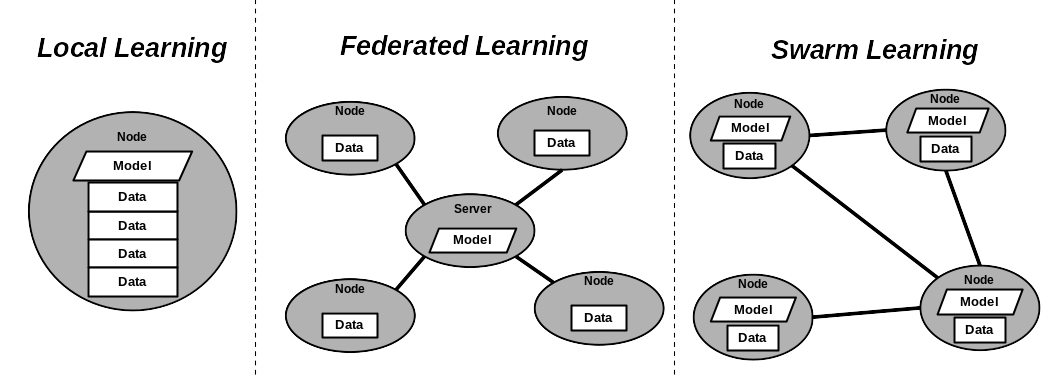
\includegraphics[width=\linewidth]{fedvsswarm}
	\caption{Diagram of different learning algorithms. Each \emph{Node} indicates a single training machine, and each line denotes a connection between two machines, along which the model can be shared. In the swarm learning diagram, the dashed lines show that each local model is an approximation of the global model.} \label{fig_learning}
\end{figure}

One SL algorithm, referred to by this paper as SwarmBC, uses a blockchain to store the global model \cite{swarm_learning}. In this version of SL, training is performed by repeating the following steps:
\begin{enumerate}
	\item A node obtains a copy of the global model from the blockchain.
	\item The node performs some training with their copy of the model and their own private data.
	\item The updated model is merged with the latest blockchain model and sent back to the blockchain for other nodes to use.
\end{enumerate}

% Specify why swarm learning is better than conventional learning or federated learning
SL exhibits many of the same benefits of FL over conventional learning, but it also improves upon FL in some aspects. As is often the case when comparing decentralised algorithms to their centralised counterparts \cite{swarm_resil}, the absence of a central server theoretically makes SL more resilient to failures than centralized FL approaches such as FedAvg. The lack of a leader election protocol also means that SL may be better suited to tasks where networks of nodes are sparsely connected, as leader election in dynamic networks is a complex problem and can add large amounts of overhead \cite{leaderelection}. Additionally, the removal of the need for a server in SL reduces the likelihood of performance bottlenecks due to network speed constraints for very large swarms.

\section{Blockchain} \label{bg:bc}
\todo{Write this out. The point of this section is to give the disadvantages of blockchain to support my idea to remove it}

% Breif intro of what a blockcahin is
Blockchain is  \todo{Short intro of what blockchain is. This does not need to be long as this is not important} \cite{blockchain_review}

% Disadvantages of using blockchain
%% Scalability
Blockchain has problems with scalability \todo{Why is blockchain hard to scale} \cite{blockchain_scale}.

%% High transaction cost
Blockchain is inefficient and slow \todo{The following paper shows that blockchain can be very slow} \cite{blockchain_scale}.